% answers.tex —— 2002 年·全国新课程卷·文科 · 参考答案与详细解析片段
% 由 tools/generate_projects.py 依来源总账自 2002/2002_数学真题_全国新课程文_试题.md + 2002/2002_数学真题_全国新课程文_解析正文.md + 2002/2002_数学真题_全国新课程文_答案要点.md 生成，勿手改（改源 MD 后重跑）


\begin{gktip}
固定源 PDF 为印刷页码 116–117 的两页题面，不附答案。以下解析均依据题面独立复算；第 13 题和第 19 题图形在 LaTeX 工程中以 TikZ/PGFPlots 矢量源重绘。
\end{gktip}

\gkpart{一、选择题}

\begin{answer}
\gksolhead{1}{}

\textbf{题目}：

直线 $(1+a)x+y+1=0$ 与圆 $x^2+y^2-2x=0$ 相切，则 $a$ 的值为\mbox{（　　）}

（A）$\pm1$　　（B）$\pm2$　　（C）$1$　　（D）$-1$

\Needspace{4\baselineskip}
\textbf{解析}

\Needspace{5\baselineskip}
圆 $x^2+y^2-2x=0$ 的圆心为 $(1,0)$、半径为 $1$。圆心到直线的距离满足

\nopagebreak[4]
\[
\frac{|(1+a)+1|}{\sqrt{(1+a)^2+1}}=1.
\]

平方并化简得 $a=-1$。

\gkanswer{答案：D}

\end{answer}
\begin{answer}
\gksolhead{2}{}

\textbf{题目}：

已知 $m\text{、}n$ 为异面直线，$m\subset$ 平面 $\alpha$，$n\subset$ 平面 $\beta$，$\alpha\cap\beta=l$，则 $l$\mbox{（　　）}

（A）与 $m\text{、}n$ 都相交

（B）与 $m\text{、}n$ 中至少一条相交

（C）与 $m\text{、}n$ 都不相交

（D）至多与 $m\text{、}n$ 中的一条相交

\Needspace{4\baselineskip}
\textbf{解析}

若 $l$ 既不与 $m$ 相交，也不与 $n$ 相交，则由于 $m\text{、}l$ 同在平面 $\alpha$ 内、$n\text{、}l$ 同在平面 $\beta$ 内，必有 $m\parallel l$ 且 $n\parallel l$，从而 $m\parallel n$，这与 $m\text{、}n$ 为异面直线矛盾。因此 $l$ 至少与 $m\text{、}n$ 中的一条相交。

\gkanswer{答案：B}

\end{answer}
\begin{answer}
\gksolhead{3}{}

\textbf{题目}：

函数 $y=a^x$ 在 $[0,1]$ 上的最大值与最小值之和为 $3$，则 $a=$\mbox{（　　）}

（A）$\dfrac12$　　（B）$2$　　（C）$4$　　（D）$\dfrac14$

\Needspace{4\baselineskip}
\textbf{解析}

若 $a>1$，函数 $a^x$ 在 $[0,1]$ 上的最小值、最大值分别为 $1\text{、}a$，故 $1+a=3$，得 $a=2$。若 $0<a<1$，最大值与最小值之和为 $1+a<2$，不可能为 $3$。

\gkanswer{答案：B}

\end{answer}
\begin{answer}
\gksolhead{4}{}

\textbf{题目}：

不等式 $(1+x)(1-|x|)>0$ 的解集是\mbox{（　　）}

（A）$\{x\mid 0\leqslant x<1\}$

（B）$\{x\mid x<0\text{ \text{且} }x\neq-1\}$

（C）$\{x\mid -1<x<1\}$

（D）$\{x\mid x<1\text{ \text{且} }x\neq-1\}$

\Needspace{4\baselineskip}
\textbf{解析}

当 $x\geqslant0$ 时，不等式化为 $(1+x)(1-x)>0$，解为 $0\leqslant x<1$；当 $x<0$ 时，化为 $(1+x)^2>0$，解为 $x<0$ 且 $x\neq-1$。合并得 $x<1$ 且 $x\neq-1$。

\gkanswer{答案：D}

\end{answer}
\begin{answer}
\gksolhead{5}{}

\textbf{题目}：

在 $(0,2\pi)$ 内，使 $\sin x>\cos x$ 成立的 $x$ 的取值范围是\mbox{（　　）}

（A）$\left(\dfrac\pi4,\dfrac\pi2\right)\cup\left(\pi,\dfrac{5\pi}4\right)$

（B）$\left(\dfrac\pi4,\pi\right)$

（C）$\left(\dfrac\pi4,\dfrac{5\pi}4\right)$

（D）$\left(\dfrac\pi4,\pi\right)\cup\left(\dfrac{5\pi}4,\dfrac{3\pi}2\right)$

\Needspace{4\baselineskip}
\textbf{解析}

\nopagebreak[4]
\[
\sin x>\cos x
\Longleftrightarrow
\sin\left(x-\frac\pi4\right)>0.
\]

在 $0<x<2\pi$ 内，解集为 $\left(\dfrac\pi4,\dfrac{5\pi}4\right)$。

\gkanswer{答案：C}

\end{answer}
\begin{answer}
\gksolhead{6}{}

\textbf{题目}：

\Needspace{5\baselineskip}
设集合

\nopagebreak[4]
\[
M=\left\{x\middle|x=\frac{k}{2}+\frac14,\ k\in\mathbb Z\right\},\qquad
N=\left\{x\middle|x=\frac{k}{4}+\frac12,\ k\in\mathbb Z\right\},
\]

则\mbox{（　　）}

（A）$M=N$　　（B）$M\subseteq N$　　（C）$M\supseteq N$　　（D）$M\cap N=\varnothing$

\Needspace{4\baselineskip}
\textbf{解析}

\nopagebreak[4]
\[
M=\left\{\frac{2k+1}{4}\middle|k\in\mathbb Z\right\},\qquad
N=\left\{\frac{j}{4}\middle|j\in\mathbb Z\right\}.
\]

因此 $M\subseteq N$。

\gkanswer{答案：B}

\end{answer}
\begin{answer}
\gksolhead{7}{}

\textbf{题目}：

椭圆 $5x^2+ky^2=5$ 的一个焦点是 $(0,2)$，那么 $k=$\mbox{（　　）}

（A）$-1$　　（B）$1$　　（C）$\sqrt5$　　（D）$-\sqrt5$

\Needspace{4\baselineskip}
\textbf{解析}

\Needspace{5\baselineskip}
将椭圆方程化为

\nopagebreak[4]
\[
x^2+\frac{k}{5}y^2=1.
\]

\Needspace{5\baselineskip}
焦点在 $y$ 轴上且焦距参数满足

\nopagebreak[4]
\[
\frac5k-1=2^2.
\]

故 $5/k=5$，所以 $k=1$。

\gkanswer{答案：B}

\end{answer}
\begin{answer}
\gksolhead{8}{}

\textbf{题目}：

正六棱柱 $ABCDEF-A_1B_1C_1D_1E_1F_1$ 的底面边长为 $1$，侧棱长为 $\sqrt2$，则这个棱柱侧面对角线 $E_1D$ 与 $BC_1$ 所成的角是\mbox{（　　）}

（A）$90^\circ$　　（B）$60^\circ$　　（C）$45^\circ$　　（D）$30^\circ$

\Needspace{4\baselineskip}
\textbf{解析}

\Needspace{5\baselineskip}
在正六棱柱底面中取边长为 $1$ 的正六边形，令竖直方向为 $z$ 轴。可取

\nopagebreak[4]
\[
\overrightarrow{E_1D}=\left(-\frac12,\frac{\sqrt3}{2},-\sqrt2\right),\qquad
\overrightarrow{BC_1}=(-1,0,\sqrt2).
\]

\Needspace{5\baselineskip}
两向量的长度均为 $\sqrt3$，且内积为 $-\dfrac32$。直线所成的角取锐角，故

\nopagebreak[4]
\[
\cos\theta=\frac{|\overrightarrow{E_1D}\cdot\overrightarrow{BC_1}|}{3}
=\frac12,
\]

所以 $\theta=60^\circ$。

\gkanswer{答案：B}

\end{answer}
\begin{answer}
\gksolhead{9}{}

\textbf{题目}：

函数 $y=x^2+bx+c$，$x\in[0,+\infty)$ 是单调函数的充要条件是\mbox{（　　）}

（A）$b\geqslant0$　　（B）$b\leqslant0$　　（C）$b>0$　　（D）$b<0$

\Needspace{4\baselineskip}
\textbf{解析}

在 $[0,+\infty)$ 上，$y'=2x+b$。要使函数单调递增，只需且必须有 $b\geqslant0$；当 $b<0$ 时导数先负后正，函数不单调。因此条件为 $b\geqslant0$。

\gkanswer{答案：A}

\end{answer}
\begin{answer}
\gksolhead{10}{}

\textbf{题目}：

已知 $0<x<y<a<1$，则有\mbox{（　　）}

（A）$\log_a(xy)<0$

（B）$0<\log_a(xy)<1$

（C）$1<\log_a(xy)<2$

（D）$\log_a(xy)>2$

\Needspace{4\baselineskip}
\textbf{解析}

\Needspace{5\baselineskip}
由 $0<x<y<a<1$ 得 $0<xy<a^2$。由于 $0<a<1$，以 $a$ 为底的对数函数递减，从而

\nopagebreak[4]
\[
\log_a(xy)>\log_a(a^2)=2.
\]

\gkanswer{答案：D}

\end{answer}
\begin{answer}
\gksolhead{11}{}

\textbf{题目}：

从正方体的 6 个面中选取 3 个面，其中有 2 个面不相邻的选法共有\mbox{（　　）}

（A）8 种　　（B）12 种　　（C）16 种　　（D）20 种

\Needspace{4\baselineskip}
\textbf{解析}

先选一对相对的面，有 $3$ 种选法；第三个面可从剩下的 $4$ 个面中任取。因此共有 $3\times4=12$ 种。

\gkanswer{答案：B}

\end{answer}
\begin{answer}
\gksolhead{12}{}

\textbf{题目}：

\Needspace{5\baselineskip}
平面直角坐标系中，$O$ 为坐标原点，已知两点 $A(3,1)\text{、}B(-1,3)$，若点 $C$ 满足

\nopagebreak[4]
\[
\overrightarrow{OC}=\alpha\overrightarrow{OA}+\beta\overrightarrow{OB},
\qquad \alpha,\beta\in\mathbb R,\quad \alpha+\beta=1,
\]

则点 $C$ 的轨迹方程为\mbox{（　　）}

（A）$3x+2y-11=0$

（B）$(x-1)^2+(y-2)^2=5$

（C）$2x-y=0$

（D）$x+2y-5=0$

\Needspace{4\baselineskip}
\textbf{解析}

\Needspace{5\baselineskip}
设 $C=(x,y)$。由 $\alpha+\beta=1$，

\nopagebreak[4]
\[
(x,y)=\alpha(3,1)+(1-\alpha)(-1,3)
=(4\alpha-1,3-2\alpha).
\]

\Needspace{5\baselineskip}
消去 $\alpha$ 得

\nopagebreak[4]
\[
x+2y-5=0.
\]

\gkanswer{答案：D}

\end{answer}
\gkpart{二、填空题}

\begin{answer}
\gksolhead{13}{}

\textbf{题目}：

据新华社 2002 年 3 月 12 日电，1985 年到 2000 年间，我国农村人均居住面积如图所示，其中，从\gkblank{}年到\gkblank{}年的五年间增长最快。
\nopagebreak[4]
\begin{center}% 2002 年全国新课程文科第 13 题：农村人均居住面积折线图
\begin{tikzpicture}[x=0.9cm,y=0.25cm,>=stealth]
  \draw[->] (0,0)--(10.5,0) node[right] {年份};
  \draw[->] (0,0)--(0,31) node[above] {面积/$\mathrm{m^2}$};
  \foreach \y/\label in {10/10,15/15,20/20,25/25,30/30}
    \draw (-0.12,\y)--(0.12,\y) node[left=5pt] {\label};
  \foreach \x/\label in {1/1985,4/1990,7/1995,10/2000}
    \draw (\x,0.15)--(\x,-0.15) node[below=4pt] {\label};
  \draw[thick] (1,14.7)--(4,17.8)--(7,21.0)--(10,24.8);
  \foreach \x/\y/\label in {
    1/14.7/14.7,
    4/17.8/17.8,
    7/21.0/21.0,
    10/24.8/24.8}
  {
    \fill (\x,\y) circle (1.4pt);
    \node[above=3pt] at (\x,\y) {\label};
  }
\end{tikzpicture}
\end{center}
\nopagebreak[4]
\begin{center}
\begin{tabular}{lrrrr}
\toprule
年份 & 1985 & 1990 & 1995 & 2000 \\
\midrule
人均居住面积（$\mathrm{m^2}$） & 14.7 & 17.8 & 21.0 & 24.8 \\
\bottomrule
\end{tabular}
\end{center}

\Needspace{4\baselineskip}
\textbf{解析}

\Needspace{5\baselineskip}
相邻五年的人均居住面积增长量分别为

\nopagebreak[4]
\[
17.8-14.7=3.1,\qquad
21.0-17.8=3.2,\qquad
24.8-21.0=3.8.
\]

最大增长量出现在 1995 年到 2000 年。

\gkanswer{答案：1995—2000}

\end{answer}
\begin{answer}
\gksolhead{14}{}

\textbf{题目}：

已知 $\sin2\alpha=-\sin\alpha$，$\alpha\in\left(\dfrac\pi2,\pi\right)$，则 $\cot\alpha=$\gkblank{}。

\Needspace{4\baselineskip}
\textbf{解析}

\Needspace{5\baselineskip}
因 $\alpha\in(\pi/2,\pi)$，$\sin\alpha\neq0$。由

\nopagebreak[4]
\[
\sin2\alpha=-\sin\alpha
\Longrightarrow
2\sin\alpha\cos\alpha=-\sin\alpha
\]

\Needspace{5\baselineskip}
得 $\cos\alpha=-\dfrac12$。又 $\sin\alpha=\dfrac{\sqrt3}{2}$，所以

\nopagebreak[4]
\[
\cot\alpha=-\frac{\sqrt3}{3}.
\]

\gkanswer{答案：$-\dfrac{\sqrt3}{3}$}

\end{answer}
\begin{answer}
\gksolhead{15}{}

\textbf{题目}：

甲、乙两种冬小麦试验品种连续 5 年的平均单位面积产量如下（单位：$\mathrm{t/km^2}$）：

\begin{center}
\begin{tabular}{lrrrrr}
\toprule
品种 & 第 1 年 & 第 2 年 & 第 3 年 & 第 4 年 & 第 5 年 \\
\midrule
甲 & 9.8 & 9.9 & 10.1 & 10.0 & 10.2 \\
乙 & 9.4 & 10.3 & 10.8 & 9.7 & 9.8 \\
\bottomrule
\end{tabular}
\end{center}

其中产量比较稳定的小麦品种是\gkblank{}。

\Needspace{4\baselineskip}
\textbf{解析}

甲的平均产量为 $10$，离均值的偏差为 $-0.2,-0.1,0.1,0,0.2$；乙的平均产量也为 $10$，离均值的偏差为 $-0.6,0.3,0.8,-0.3,-0.2$。甲的偏差整体更小，故甲的产量比较稳定。

\gkanswer{答案：甲}

\end{answer}
\begin{answer}
\gksolhead{16}{}

\textbf{题目}：

设函数 $f(x)$ 在 $(-\infty,+\infty)$ 内有定义，下列函数

① $y=-|f(x)|$；② $y=xf(x^2)$；③ $y=-f(-x)$；④ $y=f(x)-f(-x)$。

其中必为奇函数的有\gkblank{}。（要求填写正确答案的序号）

\Needspace{4\baselineskip}
\textbf{解析}

\Needspace{5\baselineskip}
① $-|f(x)|$ 为偶函数而不一定为奇函数；② $f(x^2)$ 是偶函数，乘以 $x$ 后必为奇函数；③ $-f(-x)$ 不一定具有奇偶性；④

\nopagebreak[4]
\[
f(-x)-f(x)=-(f(x)-f(-x)),
\]

故④必为奇函数。因此应填②④。

\gkanswer{答案：②④}

\end{answer}
\gkpart{三、解答题}

\begin{answer}
\gksolhead{17}{}

\textbf{题目}：

在等比数列 $\{a_n\}$ 中，已知 $a_6-a_4=24$，$a_3a_5=64$，求 $\{a_n\}$ 前 8 项的和 $S_8$。

\Needspace{4\baselineskip}
\textbf{解析}

\Needspace{5\baselineskip}
设等比数列的公比为 $q$。由等比数列性质

\nopagebreak[4]
\[
a_3a_5=a_4^2=64,
\]

\Needspace{5\baselineskip}
所以 $a_4=\pm8$。又

\nopagebreak[4]
\[
a_6-a_4=a_4(q^2-1)=24.
\]

若 $a_4=-8$，则 $q^2=-2$，不可能；故 $a_4=8$，从而 $q^2=4$，即 $q=2$ 或 $q=-2$。

\Needspace{5\baselineskip}
当 $q=2$ 时，$a_1=1$，所以

\nopagebreak[4]
\[
S_8=1+2+4+\cdots+2^7=255.
\]

\Needspace{5\baselineskip}
当 $q=-2$ 时，$a_1=-1$，所以

\nopagebreak[4]
\[
S_8=-1+2-4+8-16+32-64+128=85.
\]

\gkanswer{答案：$S_8=255$ 或 $S_8=85$。若另加公比为正的约定，则取 $255$。}

\end{answer}
\begin{answer}
\gksolhead{18}{}

\textbf{题目}：

已知 $\sin^2 2\alpha+\sin2\alpha\cos\alpha-\cos2\alpha=1$，$\alpha\in\left(0,\dfrac\pi2\right)$，求 $\sin\alpha\text{、}\tan\alpha$ 的值。

\Needspace{4\baselineskip}
\textbf{解析}

\Needspace{5\baselineskip}
令 $s=\sin\alpha$、$c=\cos\alpha$。因 $\alpha\in(0,\pi/2)$，有 $s,c>0$。原式化为

\nopagebreak[4]
\[
4s^2c^2+2sc^2-(c^2-s^2)=1.
\]

\Needspace{5\baselineskip}
利用 $s^2+c^2=1$ 整理得

\nopagebreak[4]
\[
2c^2(2s^2+s-1)=0.
\]

\Needspace{5\baselineskip}
因 $c\neq0$，故 $2s^2+s-1=0$。取正根得 $s=\dfrac12$，于是 $c=\dfrac{\sqrt3}{2}$，从而

\nopagebreak[4]
\[
\sin\alpha=\frac12,\qquad \tan\alpha=\frac{\sqrt3}{3}.
\]

\gkanswer{答案：$\sin\alpha=\dfrac12$，$\tan\alpha=\dfrac{\sqrt3}{3}$。}

\end{answer}
\begin{answer}
\gksolhead{19}{}

\textbf{题目}：

【甲】正三棱柱 $ABC-A_1B_1C_1$ 的底面边长为 $a$，侧棱长为 $\sqrt2a$。
\nopagebreak[4]
\begin{center}% 2002 年全国新课程文科第 19 题甲：正三棱柱
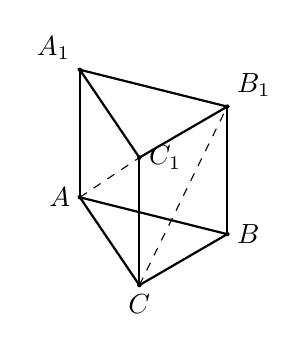
\begin{tikzpicture}[>=stealth,scale=0.72]
  \coordinate (A) at (0,0);
  \coordinate (B) at (2.6,-0.65);
  \coordinate (C) at (1.05,-1.55);
  \coordinate (Aone) at (0,2.25);
  \coordinate (Bone) at (2.6,1.60);
  \coordinate (Cone) at (1.05,0.70);
  \draw[thick] (A)--(B)--(C)--cycle;
  \draw[thick] (Aone)--(Bone)--(Cone)--cycle;
  \draw[thick] (A)--(Aone) (B)--(Bone) (C)--(Cone);
  \draw[dashed] (A)--(Cone) (C)--(Bone);
  \fill (A) circle (1.1pt) node[left] {$A$};
  \fill (B) circle (1.1pt) node[right] {$B$};
  \fill (C) circle (1.1pt) node[below] {$C$};
  \fill (Aone) circle (1.1pt) node[above left] {$A_1$};
  \fill (Bone) circle (1.1pt) node[above right] {$B_1$};
  \fill (Cone) circle (1.1pt) node[right] {$C_1$};
\end{tikzpicture}
\end{center}
\nopagebreak[4]
（1） 建立适当的坐标系，并写出点 $A\text{、}B\text{、}A_1\text{、}C_1$ 的坐标；

（2） 求 $AC_1$ 与侧面 $ABB_1A_1$ 所成的角。

【乙】如图，正方形 $ABCD\text{、}ABEF$ 的边长都是 1，而且平面 $ABCD\text{、}ABEF$ 互相垂直。点 $M$ 在 $AC$ 上移动，点 $N$ 在 $BF$ 上移动，若 $CM=BN=a$（$0<a<\sqrt2$）。
\nopagebreak[4]
\begin{center}% 2002 年全国新课程文科第 19 题乙：两个互相垂直的正方形
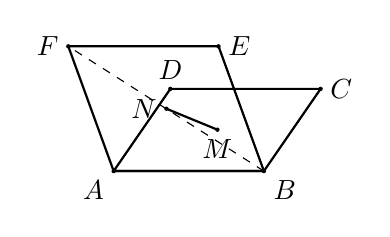
\begin{tikzpicture}[>=stealth,scale=0.72]
  \coordinate (A) at (0,0);
  \coordinate (B) at (2.65,0);
  \coordinate (C) at (3.65,1.45);
  \coordinate (D) at (1.0,1.45);
  \coordinate (E) at (1.85,2.20);
  \coordinate (F) at (-0.80,2.20);
  \coordinate (M) at (1.83,0.73);
  \coordinate (N) at (0.93,1.10);
  \draw[thick] (A)--(B)--(C)--(D)--cycle;
  \draw[thick] (A)--(B)--(E)--(F)--cycle;
  \draw[dashed] (A)--(D) (B)--(F);
  \draw[thick] (M)--(N);
  \fill (A) circle (1.1pt) node[below left] {$A$};
  \fill (B) circle (1.1pt) node[below right] {$B$};
  \fill (C) circle (1.1pt) node[right] {$C$};
  \fill (D) circle (1.1pt) node[above] {$D$};
  \fill (E) circle (1.1pt) node[right] {$E$};
  \fill (F) circle (1.1pt) node[left] {$F$};
  \fill (M) circle (1.1pt) node[below] {$M$};
  \fill (N) circle (1.1pt) node[left] {$N$};
\end{tikzpicture}
\end{center}
\nopagebreak[4]
（1） 求 $MN$ 的长；

（2） $a$ 为何值时，$MN$ 的长最小；

（3） 当 $MN$ 的长最小时，求面 $MNA$ 与面 $MNB$ 所成二面角 $\alpha$ 的大小。

\Needspace{10\baselineskip}
\textbf{解析}

\textbf{甲}

\gksubpart{(1)}

\Needspace{5\baselineskip}
取 $A=(0,0,0)$、$B=(a,0,0)$，令正三角形 $ABC$ 位于 $xOy$ 平面，令侧棱方向为 $z$ 轴，则

\nopagebreak[4]
\[
C=\left(\frac a2,\frac{\sqrt3a}{2},0\right),\qquad
A_1=(0,0,\sqrt2a),
\]

\Needspace{5\baselineskip}
以及

\nopagebreak[4]
\[
B_1=(a,0,\sqrt2a),\qquad
C_1=\left(\frac a2,\frac{\sqrt3a}{2},\sqrt2a\right).
\]

\gksubpart{(2)}

\Needspace{5\baselineskip}
侧面 $ABB_1A_1$ 的方程为 $y=0$。方向向量

\nopagebreak[4]
\[
\overrightarrow{AC_1}
=\left(\frac a2,\frac{\sqrt3a}{2},\sqrt2a\right),
\qquad
|\overrightarrow{AC_1}|=\sqrt3a.
\]

\Needspace{5\baselineskip}
设直线与平面的夹角为 $\theta$，则

\nopagebreak[4]
\[
\sin\theta
=\frac{\left|\frac{\sqrt3a}{2}\right|}{\sqrt3a}
=\frac12,
\]

所以 $\theta=\dfrac\pi6$。

\textbf{乙}

\gksubpart{(1)}

\Needspace{5\baselineskip}
取

\nopagebreak[4]
\[
A=(0,0,0),\quad B=(1,0,0),\quad C=(1,1,0),\quad D=(0,1,0),
\]

\Needspace{5\baselineskip}
并令

\nopagebreak[4]
\[
E=(1,0,1),\qquad F=(0,0,1).
\]

\Needspace{5\baselineskip}
设 $t=a/\sqrt2$。由 $CM=a$、$BN=a$，

\nopagebreak[4]
\[
M=(1-t,1-t,0),\qquad N=(1-t,0,t).
\]

\Needspace{5\baselineskip}
于是

\nopagebreak[4]
\[
MN^2=(1-t)^2+t^2
=a^2-\sqrt2a+1,
\]

\Needspace{5\baselineskip}
即

\nopagebreak[4]
\[
MN=\sqrt{a^2-\sqrt2a+1}.
\]

\gksubpart{(2)}

\Needspace{5\baselineskip}
配方得

\nopagebreak[4]
\[
MN^2=\left(a-\frac{\sqrt2}{2}\right)^2+\frac12.
\]

所以当 $a=\dfrac{\sqrt2}{2}$ 时，$MN$ 取得最小值 $\dfrac{\sqrt2}{2}$。

\gksubpart{(3)}

\Needspace{5\baselineskip}
此时 $t=\dfrac12$，故

\nopagebreak[4]
\[
M=\left(\frac12,\frac12,0\right),\qquad
N=\left(\frac12,0,\frac12\right).
\]

\Needspace{5\baselineskip}
可验证 $\triangle AMN$ 与 $\triangle BMN$ 都是边长 $\dfrac{\sqrt2}{2}$ 的正三角形。设 $H$ 为 $MN$ 的中点，则 $AH\perp MN$、$BH\perp MN$，所以所求二面角的平面角为 $\angle AHB$。有

\nopagebreak[4]
\[
\overrightarrow{HA}=\left(-\frac12,-\frac14,-\frac14\right),\qquad
\overrightarrow{HB}=\left(\frac12,-\frac14,-\frac14\right),
\]

\Needspace{5\baselineskip}
从而

\nopagebreak[4]
\[
\cos\angle AHB
=\frac{-1/8}{(3/8)}
=-\frac13.
\]

因此二面角 $\alpha=\arccos\left(-\dfrac13\right)$。

\gkanswer{答案（1）：甲：坐标见解析版；乙：$MN=\sqrt{a^2-\sqrt2a+1}$。}

\gkanswer{答案（2）：甲：$\dfrac\pi6$；乙：$a=\dfrac{\sqrt2}{2}$。}

\gkanswer{答案（3）：甲：无此小问；乙：$\alpha=\arccos\left(-\dfrac13\right)$。}

\end{answer}
\begin{answer}
\gksolhead{20}{}

\textbf{题目}：

某单位 6 个员工借助互联网开展工作，每个员工上网的概率都是 0.5（相互独立）。

（1） 求至少 3 人同时上网的概率；

（2） 至少几人同时上网的概率小于 0.3？

\Needspace{4\baselineskip}
\textbf{解析}

设上网人数为 $X$，则 $X\sim B(6,0.5)$。

\gksubpart{(1)}

\nopagebreak[4]
\[
P(X\geqslant3)
=\frac{\binom63+\binom64+\binom65+\binom66}{2^6}
=\frac{20+15+6+1}{64}
=\frac{21}{32}.
\]

\gksubpart{(2)}

\nopagebreak[4]
\[
P(X\geqslant4)=\frac{15+6+1}{64}=\frac{22}{64}>0.3,
\]

\Needspace{5\baselineskip}
而

\nopagebreak[4]
\[
P(X\geqslant5)=\frac{6+1}{64}=\frac7{64}<0.3.
\]

所以至少 5 人同时上网时，该概率小于 $0.3$。

\gkanswer{答案（1）：$\dfrac{21}{32}$。}

\gkanswer{答案（2）：5 人。}

\end{answer}
\begin{answer}
\gksolhead{21}{}

\textbf{题目}：

已知 $a>0$，函数 $f(x)=x^3-a$，$x\in(0,+\infty)$。设 $x_1>0$，记曲线 $y=f(x)$ 在点 $(x_1,f(x_1))$ 处的切线为 $l$。

（1） 求 $l$ 的方程；

（2） 设 $l$ 与 $x$ 轴交点为 $(x_2,0)$。证明：

① $x_2\geqslant\sqrt[3]{a}$；

② 若 $x_2>\sqrt[3]{a}$，则 $\sqrt[3]{a}<x_2<x_1$。

\Needspace{4\baselineskip}
\textbf{解析}

\gksubpart{(1)}

\nopagebreak[4]
\[
f'(x)=3x^2.
\]

\Needspace{5\baselineskip}
切线方程为

\nopagebreak[4]
\[
y-(x_1^3-a)=3x_1^2(x-x_1),
\]

\Needspace{5\baselineskip}
即

\nopagebreak[4]
\[
y=3x_1^2x-2x_1^3-a.
\]

\gksubpart{(2)}

\Needspace{5\baselineskip}
令 $y=0$，得到切线与 $x$ 轴交点的横坐标

\nopagebreak[4]
\[
x_2=\frac{2x_1^3+a}{3x_1^2}
=\frac{2x_1}{3}+\frac{a}{3x_1^2}.
\]

\Needspace{5\baselineskip}
设 $r=\sqrt[3]{a}$。加权算术—几何平均不等式给出

\nopagebreak[4]
\[
x_2=\frac{2x_1+x_1\cdot\frac{a}{x_1^3}}3
\geqslant
\sqrt[3]{x_1^2\cdot\frac{a}{x_1^2}}
=r.
\]

\Needspace{5\baselineskip}
这证明了①。另一方面，

\nopagebreak[4]
\[
x_2-x_1=\frac{a-x_1^3}{3x_1^2}.
\]

因此只有在 $x_1>r$ 时才有 $x_2<x_1$；当 $0<x_1<r$ 时，反而有 $x_2>x_1$。例如 $a=1\text{、}x_1=\dfrac12$ 时，$x_2=\dfrac32$，所以固定源中的②按字面并不成立。若②的前提原拟写为 $x_1>\sqrt[3]{a}$，则由上式与①即可得到 $\sqrt[3]{a}<x_2<x_1$。

\gkanswer{答案（1）：$l:y=3x_1^2x-2x_1^3-a$。}

\gkanswer{答案（2）：$x_2=\dfrac{2x_1}{3}+\dfrac{a}{3x_1^2}\geqslant\sqrt[3]{a}$；第②问按题面不成立，例如 $a=1,x_1=\dfrac12$ 时 $x_2=\dfrac32>1$ 但 $x_2>x_1$。若原题拟补条件 $x_1>\sqrt[3]{a}$，则 $\sqrt[3]{a}<x_2<x_1$。}

\end{answer}
\begin{answer}
\gksolhead{22}{}

\textbf{题目}：

已知两点 $M(-1,0)\text{、}N(1,0)$，且点 $P$ 使 $\overrightarrow{MP}\cdot\overrightarrow{MN}$、$\overrightarrow{PM}\cdot\overrightarrow{PN}$、$\overrightarrow{NM}\cdot\overrightarrow{NP}$ 成公差小于零的等差数列。

（1） 点 $P$ 的轨迹是什么曲线？

（2） 若点 $P$ 坐标为 $(x_0,y_0)$，记 $\theta$ 为 $\overrightarrow{PM}$ 与 $\overrightarrow{PN}$ 的夹角，求 $\tan\theta$。

\Needspace{4\baselineskip}
\textbf{解析}

\gksubpart{(1)}

\Needspace{5\baselineskip}
设 $P=(x,y)$。记三个数量为

\nopagebreak[4]
\[
u=\overrightarrow{MP}\cdot\overrightarrow{MN}=2(x+1),
\]

\nopagebreak[4]
\[
v=\overrightarrow{PM}\cdot\overrightarrow{PN}=x^2+y^2-1,
\]

\nopagebreak[4]
\[
w=\overrightarrow{NM}\cdot\overrightarrow{NP}=2(1-x).
\]

\Needspace{5\baselineskip}
因 $u,v,w$ 成等差数列，故 $u+w=2v$，即

\nopagebreak[4]
\[
4=2(x^2+y^2-1),
\qquad\text{\text{从而}}\qquad
x^2+y^2=3.
\]

\Needspace{5\baselineskip}
等差数列的公差为

\nopagebreak[4]
\[
w-v=2(1-x)-2=-2x.
\]

公差小于零要求 $x>0$。因此轨迹是圆 $x^2+y^2=3$ 的右半圆。

\gksubpart{(2)}

\Needspace{5\baselineskip}
又在该轨迹上 $\overrightarrow{PM}\cdot\overrightarrow{PN}=2$，而两向量叉积的绝对值为 $2|y|$，故

\nopagebreak[4]
\[
\tan\theta
=\frac{2|y_0|}{2}
=|y_0|.
\]

\gkanswer{答案（1）：圆 $x^2+y^2=3$ 的右半圆（$x>0$）。}

\gkanswer{答案（2）：$\tan\theta=|y_0|$。}

\end{answer}
